\section{Applications of Integrals}

Many applications of integrals use the following heuristic idea: you have a value $A$ that you want to compute; you break the problem up into infinitesimal pieces and compute the corresponding infinitesimal value ''$dA$''; then sum up the small values by integrating
$$A=\int\ dA.$$

Understanding integrals as sums will make understanding these integral applications easier.
The first example of this you will see is computing areas. \mar{Try to find all such examples.}

\subsection{Average Values}

The average value of $f$ on $[a,b]$ is 
$$\frac{\displaystyle\int_a^bf(x)\ dx}{b-a}.$$
There are various intuitive explanations of this; here are two.

\subsubsection{Water in a tank}
Imagine water is sloshing around in a tank and the height of the water at a particular time is described by a function $f(x)$ (see the figure below). 

\begin{figure}[H]
\centering

\phantom{}
\vspace{1em}



\tikzset{every picture/.style={line width=0.75pt}} %set default line width to 0.75pt        

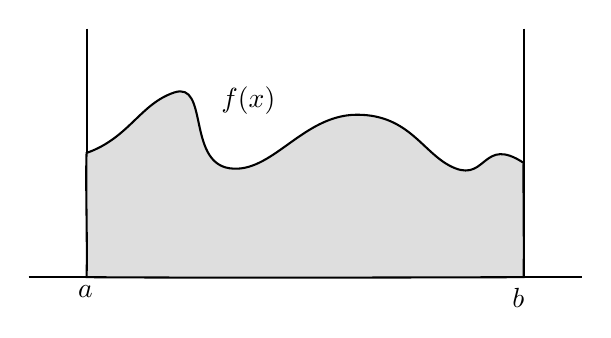
\begin{tikzpicture}[x=0.75pt,y=0.75pt,yscale=-1,xscale=1]
%uncomment if require: \path (0,409); %set diagram left start at 0, and has height of 409

%Straight Lines [id:da044590240587294216] 
\draw    (109.67,150.03) -- (376,150.03) ;
%Straight Lines [id:da5673860317913473] 
\draw    (137.55,30.33) -- (137.55,150.03) ;
%Shape: Polygon Curved [id:ds7088187846595497] 
\draw  [fill={rgb, 255:red, 222; green, 222; blue, 222 }  ,fill opacity=1 ] (179.85,61.03) .. controls (196.34,55.58) and (185.98,94.48) .. (206.35,97.55) .. controls (226.71,100.62) and (241.59,71.86) .. (267.7,71.77) .. controls (293.81,71.67) and (299.9,91.52) .. (315.11,97.55) .. controls (330.32,103.59) and (328.57,82.06) .. (348.09,94.95) .. controls (347.87,101.17) and (348.41,132.15) .. (348.11,150.03) .. controls (249.57,150.34) and (179.85,150.34) .. (137.55,150.03) .. controls (138,133) and (137,104) .. (137.55,90.18) .. controls (158,83) and (163.37,66.47) .. (179.85,61.03) -- cycle ;
%Straight Lines [id:da25646989795162733] 
\draw [color={rgb, 255:red, 0; green, 0; blue, 0 }  ,draw opacity=1 ]   (348.11,30.33) -- (348.11,150.03) ;

% Text Node
\draw (132.02,152.57) node [anchor=north west][inner sep=0.75pt]    {$a$};
% Text Node
\draw (341.18,154.1) node [anchor=north west][inner sep=0.75pt]    {$b$};
% Text Node
\draw (201.02,56.84) node [anchor=north west][inner sep=0.75pt]    {$f( x)$};


\end{tikzpicture}
\vspace{1em}

\phantom{}

\end{figure}

The average value of $f(x)$ on $[a,b]$ is the height of the water once it settles. To find this height, find the area of the water $\left(\displaystyle\int_a^bf(x)\ dx\right)$ and divide by the width of the tank ($b-a$).

\subsubsection{Using the FTC and Average Slope}
Let $F$ be an antiderivative of $f$. Then the average value of $f(x)$ on $[a,b]$ is equal to the average value of $F'$ on $[a,b]$. We know how to calculate this using the slope of a secant line:
$$\frac{F(b)-F(a)}{b-a}\overset{FTC}{=}\frac{\int_a^bf(x) \ dx}{b-a}.$$


% \subsection{Reimann Sums}
% The average of $f$ on a finite set $A=\{x_1,\dots, x_n\}$ is the sum of $f(x)$ evaluated at every element of $A$, divided by the number of elements of $A$:
% $$\frac{\sum_{i=1}^nf(x_i)}{n}.$$
\mar{Use Reimann sums to get another explanation.}


\subsection{Areas}
To compute the area $A$ between $f(x)$ and $g(x)$ on $[a,b]$, imagine dividing up the area into infinitesimally small strips, each with height $f(x)-g(x)$ and (infinitesimal) width $dx$. The area of the strip is therefore $dA=(f(x)-g(x))\ dx$. One such strip is shown on the graph below (the width enlarged to be visible). To compute the desired area, simply integrate $dA$ over $[a,b]$:
$$A=\int dA = \int_a^b(f(x)-g(x))\ dx.$$

\begin{figure}[H]
\centering

\tikzset{every picture/.style={line width=0.75pt}} %set default line width to 0.75pt        

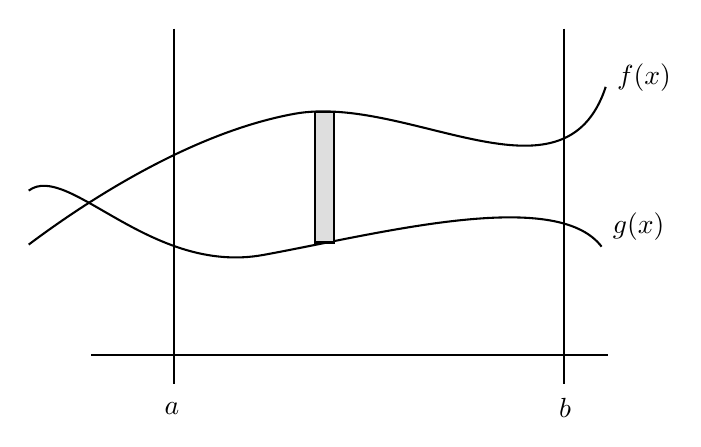
\begin{tikzpicture}[x=0.75pt,y=0.75pt,yscale=-1,xscale=1]
%uncomment if require: \path (0,300); %set diagram left start at 0, and has height of 300

%Straight Lines [id:da5705104580473277] 
\draw    (182,27) -- (182,198) ;
%Straight Lines [id:da838729158622765] 
\draw    (370,27) -- (370,198) ;
%Straight Lines [id:da13279837061190713] 
\draw    (391,184) -- (142,184) ;
%Curve Lines [id:da08034929661214907] 
\draw    (112,131) .. controls (130.83,116.88) and (185.53,77.9) .. (240,68) .. controls (294.47,58.1) and (370,116) .. (390,55) ;
%Curve Lines [id:da13490737944947462] 
\draw    (112,105) .. controls (130.83,90.88) and (170.53,145.9) .. (225,136) .. controls (279.47,126.1) and (366,103) .. (388,132) ;
%Shape: Rectangle [id:dp8230016382923657] 
\draw  [fill={rgb, 255:red, 222; green, 222; blue, 222 }  ,fill opacity=1 ] (250,67) -- (259,67) -- (259,130) -- (250,130) -- cycle ;

% Text Node
\draw (394,42.4) node [anchor=north west][inner sep=0.75pt]    {$f( x)$};
% Text Node
\draw (392,114.4) node [anchor=north west][inner sep=0.75pt]    {$g( x)$};
% Text Node
\draw (176,205.4) node [anchor=north west][inner sep=0.75pt]    {$a$};
% Text Node
\draw (366,203.4) node [anchor=north west][inner sep=0.75pt]    {$b$};

\end{tikzpicture}

\end{figure}



\subsection{Arc Length}

The \textbf{arc length} of $f(x)$ on $[a,b]$ is the length of string needed to trace the graph of $f$ on the interval $[a,b]$. Similarly to computing areas, to compute the arc length $L$ of a function $f$'s graph, divide the length into infinitesimally short segments (that we assume to be linear). Then each segment's length can be computed using the pythagorean theorem (see picture below): 
$$dL=\sqrt{dx^2+dy^2}=\sqrt{1+\frac{dy^2}{dx^2}}\ dx=\sqrt{1+f'(x)^2}\ dx.$$
Then to compute the arc length $L$, sum $dL$ over $[a,b]$ by integrating:
$$L=\int_a^b\sqrt{1+f'(x)^2}\ dx.$$

\begin{figure}[H]
\centering

\tikzset{every picture/.style={line width=0.75pt}} %set default line width to 0.75pt        

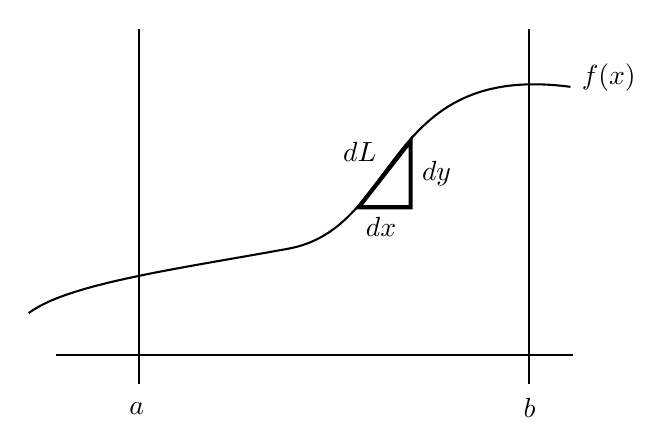
\begin{tikzpicture}[x=0.75pt,y=0.75pt,yscale=-1,xscale=1]
%uncomment if require: \path (0,300); %set diagram left start at 0, and has height of 300

%Straight Lines [id:da8511908828152182] 
\draw    (202,47) -- (202,218) ;
%Straight Lines [id:da8667346744151081] 
\draw    (390,47) -- (390,218) ;
%Straight Lines [id:da41300492628810637] 
\draw    (411,204) -- (162,204) ;
%Curve Lines [id:da05101594018896982] 
\draw    (149,184) .. controls (167.83,169.88) and (219.53,162.9) .. (274,153) .. controls (328.47,143.1) and (319,63) .. (410,75) ;
%Shape: Triangle [id:dp7671239003370118] 
\draw  [line width=1.5]  (333,101) -- (333,133) -- (308,133) -- cycle ;

% Text Node
\draw (414,62.4) node [anchor=north west][inner sep=0.75pt]    {$f( x)$};
% Text Node
\draw (196,225.4) node [anchor=north west][inner sep=0.75pt]    {$a$};
% Text Node
\draw (386,223.4) node [anchor=north west][inner sep=0.75pt]    {$b$};
% Text Node
\draw (310,136.4) node [anchor=north west][inner sep=0.75pt]    {$dx$};
% Text Node
\draw (337,109.4) node [anchor=north west][inner sep=0.75pt]    {$dy$};
% Text Node
\draw (299,100.4) node [anchor=north west][inner sep=0.75pt]    {$dL$};


\end{tikzpicture}

\end{figure}





\subsection{Probability}

Imagine we have an experiment, and every time it is performed the outcome is a real number. (Think throwing a dart at the plane, and the outcome is the $x$ coordinate of the point it lands on). 

To start, the we will define an \textbf{event} to be a subset of $\R$. Given such a subset $A\subset\R$, our goal is to describe the probability that the outcome $X$ is in $A$. We denote this $\P(X\in A)$.


For the kinds of experiments we will consider, we will assume that it is never possible to get the same outcome twice. This means that the probability of any \textit{particular} outcome is 0: for any $a\in\R$, $$\P(X\in\{a\})=\P(X=a)=0.$$ 
This might seem paradoxical, because the dart must hit \textit{some} point. However, it should make sense since there are infinitely many possible outcomes.
\mar{Think about this carefully.}

To compute $\P(X\in A)$ in general, we need a way to describe an allocation of probability specific to the experiment that is happening. For this (of course) we use a a function! A bounded function $f:\R \to \R$ is called a \textbf{probability density function} (PDF) if it is non-negative and $\int_{\infty}^\infty f(x)\ dx= 1$.\mar{What does the condition $$\int_{\infty}^\infty f(x)\ dx= 1$$ mean in terms of probability?} 
To compute a probability, we just have to integrate:
$$\P(X\in A) = \int_A f(x)\ dx.$$
This notation means that if $A$ is the union of disjoint intervals, integrate over each interval and add the results. In particular, if $A=(a,b)$, then 
$$\P(X\in A) = \int_a^b f(x)\ dx.$$
The anti-derivative function
$$F(x)=\P(X<x) = \int_{-\infty}^x f(t)\ dt$$
is called the \textbf{cumulative distribution function} (CDF).

Two statistics often used in probability are the \textbf{expected value} and the \textbf{variance}. The expected value of a PDF (if it exists) is the average value of an outcome. In finite cases, we compute the average of a finite data set with $n$ elements
$$\{\underbrace{x_1,\dots, x_1}_{a_1}, \underbrace{x_2,\dots, x_2}_{a_2},\dots, \underbrace{x_k,\dots, x_k}_{a_k}\}$$
by computing
$$\mu=\frac{1}{n}\sum_{i=1}^ka_ix_i=\sum_{i=1}^k\frac{a_i}{n}x_i =\sum_{i=1}^k\P(x_i)x_i,$$
the sum of the unique elements, each multiplied by its probability of occurring in the data set. In the continuous case we analogously compute the expected value as 
$$\mu=\int_{-\infty}^\infty xf(x)\ dx.$$

The variance of a PDF (if it exists) is the average squared distance of an outcome from the expected value. Therefore the variance is computes as
$$\sigma^2 = \int_{-\infty}^\infty (x-\mu)^2f(x)\ dx.$$
The square root of the variance is called the \textbf{standard deviation}.

Here are some examples:
\begin{itemize}
\item The ``uniform'' PDF on $(0,1)$ is defined as
$$f(x)=\begin{cases}0 & x < 0\\ 1 & 0\leq x\leq 1\\ 0 & x>1\end{cases}
\quad\quad\text{ and } \quad\quad
F(x)=\begin{cases}0 & x < 0\\ x & 0\leq x\leq 1\\ 1 & x>1\end{cases}$$
is its CDF. The probability that an outcome of an experiment governed by this PDF is greater than $1/4$ is
$$\P\left(X\in(1/4,\infty)\right)
= \int_{\frac14}^{\infty}f(x)\ dx
= \int_{\frac14}^{1}1\ dx + \int_{1}^{\infty}0\ dx 
= \frac34.
$$
The probability that an outcome is in $(0,1/2)\cup(2/3,1)$ is
$$\P\left(X\in(0,1/2)\cup(2/3,1)\right)
= \int_0^{\frac12}1\ dx + \int_{\frac23}^11\ dx
= \frac12+\frac13 = \frac56.
$$

The expected value of the uniform PDF is
$$\mu=\int_{0}^1 x\ dx=\frac{1}{2},$$
and the variance is
$$\sigma^2 = \int_{0}^1 \left(x-\frac{1}{2}\right)^2\ dx=\frac{1}{12}.$$

\item  The ``exponential'' PDF is defined as
$$f(x)=\begin{cases}0 & x < 0\\ e^{-x} & x\geq 0\end{cases}
\quad\quad\text{ and } \quad\quad
F(x)=\begin{cases}0 & x < 0\\1- e^{-x} & x\geq 0\end{cases}$$
is its CDF. This PDF is often used to model the wait time between phone calls. The probability that an outcome of an experiment governed by this PDF is greater than $1/4$ is
$$\P\left(X\in(1/4,\infty)\right)
= \int_{\frac14}^{\infty} e^{-x}\ dx
= e^{-\frac{1}{4}}.
$$
The expected value of the uniform PDF is
$$\mu=\int_{0}^\infty xe^x\ dx=1,$$
and the variance is
$$\sigma^2 = \int_{0}^\infty \left(x-1\right)^2e^{-x}\ dx=1.$$

\end{itemize}


\mar{Draw a picture of these PDFs and CDFs.}



\subsection{Volumes and Surface Area}


\subsection{Work}
